\documentclass[11pt,letterpaper]{article}
\usepackage{url}
\usepackage[numbers,sort&compress]{natbib}
% \usepackage[latin1]{inputenc} % now, we use XeLaTeX to compile this file.
\usepackage{amsmath}
\usepackage{amsfonts}
\usepackage{graphicx}
\usepackage{float}
\usepackage{xcolor}
% \usepackage{fullpage}

\usepackage[letterpaper,
            top=0.5in,
            bottom=0.5in,
            left=1in,
            right=1in,
            includefoot]{geometry}
\begin{document}

\title{LLM Driven Reinforcement Learning for ARC}

\author{
% Author names (and their umich.edu emails)
\begin{tabular}{lll}
Yifan Jing(ivaning@umich.edu) & Zhuoyu Chen(zhuoyuc@umich.edu) \\
Zikai Zhou(zikaiz@umich.edu) & Danqi Hu(danqihu@umich.edu) \\
Haolun Cai(haolunca@umich.edu) &
\end{tabular}
}
\date{\today}
\maketitle



\begin{abstract}
Please write an abstract (executive summary) here in a paragraph.

{\color{red}
1 paragraph:
\begin{enumerate}
    \item Why is the problem important and interesting?
    \item What are things that are held back because your problem has not been solved yet?
    \item What are great things that could happen if you solved your problem?
\end{enumerate}
}
\end{abstract}




\section{Introduction}
{\color{red}
\begin{enumerate}
    \item Problem description and motivation.
    \item Why do you want to solve this problem?
    \item What's the impact if you can solve this problem?
\end{enumerate}
}




% Problem Statement:
Large Language Models (LLMs) have demonstrated remarkable capabilities in code generation tasks. However, they still struggle with \textbf{complex reasoning and self-correction} when generating code for novel, abstract problems. A critical limitation is that current LLMs often produce incorrect code on the first attempt and lack the ability to iteratively refine their solutions based on execution feedback.

The \textbf{Abstraction and Reasoning Corpus (ARC)} provides an ideal testbed for this challenge. ARC tasks require models to infer transformation rules from a few input-output grid examples and generate code that generalizes to unseen test inputs. Unlike conventional coding benchmarks (e.g., HumanEval, MBPP) that test memorization of common programming patterns, ARC evaluates \textbf{core reasoning and generalization abilities}---skills that remain elusive for state-of-the-art LLMs.

\paragraph{\textbf{The central problem we address is:}}

\begin{quote}
    \textit{How can we enable LLMs to learn from execution feedback and iteratively improve their code generation through reinforcement learning, particularly for tasks requiring abstract reasoning?}
\end{quote}

Specifically, we aim to answer the following research questions:

\begin{enumerate}
    \item \textbf{Can reinforcement learning improve code generation accuracy} beyond supervised fine-tuning alone, by rewarding successful execution outcomes?
    
    \item \textbf{Can a self-correction mechanism}---where models revise their code based on error messages and incorrect outputs---be effectively learned through RL?
    
    \item \textbf{What reward shaping strategies} are most effective for guiding LLMs toward correct solutions in sparse-reward environments where most generated code fails?
\end{enumerate}

This problem is significant because solving it would bridge the gap between current LLM capabilities and human-like iterative problem-solving, with broad applications in automated programming, scientific discovery, and AI-assisted reasoning.

\subsection{Significance}
% Significance:
% 1) Why is the problem important and interesting?
% 2) What are things that are held back because your problem has not been solved yet?
% 3) What are great things that could happen if you solved your problem?
ARC is designed to test whether an AI system can reason abstractly and generalize from a few examples. That is a skill that human find natural but modern machine learning struggles with. Even the most powerful large language model perform poorly on ARC problems. The tasks require discovering previse transformation rather than recognizing statistical patterns. This gap highlights the problem with modern AI systems: they lack reliable mechanisms for symbolic reasoning, self-correction, and learning from small amounts of data.

Due to the reason that this problem remains unsolved, progress is limited in many areas that depend on structured reasoning. For example, program synthsis, automated debugging, and decision-making in complex environment. Systems that rely only on pattern matching often fail when exact logic, compositional reasoning, or correctness guarantees are required.

This project addresses current limitations by integrating code generation with execution-based feedback and reinforcement learning. Rather than directly predicting answers, the model is trained to write and iteratively refine programs based on their performance. If effective, this methodology may enable AI systems to reason more robustly, adapt with minimal data, and offer more interpretable solutions for ARC and a broad spectrum of real-world reasoning challenges.





\subsection{Evaluation}
% Evaluation:
% 1) How are you going to evaluate your method/approach?
% 2) What is the evaluation metric or protocol? 
% 3) Which dataset or benchmark are you going to use?
The proposed approach is evaluated on the \textbf{Abstraction and Reasoning Corpus (ARC)}, a benchmark designed to assess abstract reasoning and generalization from a small number of examples. For each ARC task, the model is provided with the training input-output grid pairs and is required to generate a Python program that implements the inferred transformation. The generated program is executed on the training examples, and execution feedback, including runtime errors and incorrect outputs, is incorporated to enable iterative refinement. After a limited number of correction steps, the final program is evaluated on the held-out test input. Following the official ARC evaluation protocol, a task is considered successfully solved only if the predicted output grid exactly matches the ground-truth output.

The primary evaluation metric is the task success rate, defined as the proportion of ARC tasks solved correctly on the test inputs. In addition, the effectiveness of learning from execution feedback is analyzed by measuring the number of refinement iterations required before a correct program is produced and the frequency with which generated programs execute without errors. Performance is compared before and after reinforcement learning, as well as against supervised fine-tuning without iterative correction, in order to isolate the impact of reinforcement learning and execution-based feedback on reasoning and generalization.




\section{Methodology}
{\color{red}
\begin{enumerate}
    \item How are you going to solve this problem?
    \item Why should the proposed method work?
    \item Provide explanations/rationale of why you chose this specific method.
    \item Provide technical details of your approach if you are proposing a novel method.
    \item Description of the pipeline. Including a figure(e.g., block diagram) that explains the pieline will be very helpful.
\end{enumerate}
}


Compared to PPO, GRPO removes the need for a learned value function and instead uses group-relative reward normalization. This provides a stable learning signal even when absolute rewards are sparse, making GRPO particularly suitable for ARC-style program synthesis where most sampled programs fail.

We perform post-training of an instruction-following code LLM using Group Relative Policy Optimization (GRPO). Our objective is to train the model to generate executable programs for ARC tasks and to improve solutions through interaction-based feedback and self-correction. \cite{shao2024deepseekmathpushinglimitsmathematical}

Each ARC task provides training input-output grid pairs $\{(x_i, y_i)\}_{i=1}^n$ and a test input $x_{\text{test}}$. The model generates a Python program $c$ mapping $x \mapsto \hat y$. We execute $c$ on the training inputs to obtain outputs $\{\hat y_i\}$ and diagnostic feedback $\mathcal{F}$. The model may revise its code for up to $T$ iterations. The entire multi-step generation process is treated as a trajectory and optimized with GRPO.

Let $\pi_\theta$ denote the autoregressive policy. For prompt $p$, the model produces a trajectory $\tau$ (including code, feedback, and revisions):
\[
\tau \sim \pi_\theta(\cdot \mid p), \qquad 
\log \pi_\theta(\tau\mid p)=\sum_{t=1}^{|\tau|}\log \pi_\theta(a_t\mid s_t).
\]

After execution, we assign a reward
\[
R(\tau) = R_{\text{train}}(c) + \lambda_{\text{fmt}} R_{\text{fmt}}(\tau) - \lambda_{\text{err}} R_{\text{err}}(c),
\]
where $R_{\text{train}}$ measures correctness on training pairs, $R_{\text{fmt}}$ encourages well-formed executable code, and $R_{\text{err}}$ penalizes runtime errors or timeouts. A sparse version of correctness is
\[
R_{\text{train}}(c)=\mathbb{1}\big[\forall i,\; \hat y_i = y_i\big].
\]

For each prompt, we sample $K$ trajectories $\{\tau^{(k)}\}_{k=1}^K$ from $\pi_{\theta_{\text{old}}}$, compute rewards $\{R^{(k)}\}$, and form group-relative advantages:
\[
\mu_R = \frac{1}{K}\sum_{k=1}^K R^{(k)}, \quad
\sigma_R = \sqrt{\frac{1}{K}\sum_{k=1}^K (R^{(k)}-\mu_R)^2 + \epsilon}, \quad
A^{(k)} = \frac{R^{(k)}-\mu_R}{\sigma_R}.
\]

We then optimize a clipped PPO-style objective
\[
\mathcal{L}_{\text{GRPO}}(\theta)=
\mathbb{E}_{p}\!\left[
\frac{1}{K}\sum_{k=1}^K
\min\!\big(
r_\theta(\tau^{(k)})A^{(k)},
\text{clip}(r_\theta(\tau^{(k)}),1-\varepsilon,1+\varepsilon)A^{(k)}
\big)
\right],
\]
with $r_\theta(\tau)=\pi_\theta(\tau\mid p)/\pi_{\theta_{\text{old}}}(\tau\mid p)$, plus a KL penalty toward a reference model $\pi_{\text{ref}}$:
\[
\mathcal{L}(\theta)=\mathcal{L}_{\text{GRPO}}(\theta)-\beta\,\mathbb{E}[\mathrm{KL}(\pi_\theta\|\pi_{\text{ref}})].
\]

This procedure encourages trajectories that produce executable and correct programs with fewer correction steps.





\section{Related work}
{\color{red}
\begin{enumerate}
    \item What are existing methods?
    \item What are the state-of-the-art methods for this problem?
    \item How is your approach similar to other existing work?
    \item How is your approach different from the related work?
\end{enumerate}
}

The ARC benchmark aims to measure the ability to infer rules from a small number of examples (train data) and transfer them to new problems (test data), rather than achieving a high score by fitting a large amount of data on a single task.
\citet{chollet2019measureintelligence} argues that the performance of a machine learning model on a single fixed task is strongly influenced by prior knowledge and training scale, so that ARC uses grid transformations and few-shot supervision data with prior knowledge to highlight differences in generalization.
The ARC official competition guide further sets up the data and evaluation process, such as each task is provided in JSON format, a small set of training input-output pairs, and several test inputs, and the goal of ARC is how to infer the rule from train data and generate outputs from test data\citep{arcprize_guide}.

In the direction of formulating the ARC problem as a reinforcement learning (RL) problem, ARCLE provides a dedicated RL environment from ARC, because directly applying RL on grids faces a large action space, sparse rewards hard to reach, and also diverse task types.
\citet{lee2024arcleabstractionreasoningcorpus} shows that the conventional RL methods, such as proximal policy optimization (PPO), can learn on individual tasks in this framework.

Besides, some work recognizes ARC solving as analogical reasoning because the model has the ability to extract transferable knowledge from known train data, and to apply the knowledge to similar but unseen tasks.
\citet{lee2024enhancinganalogicalreasoningabstraction} compares DreamerV3 (world-model) with PPO (model-free) on ARC tasks, and reports advantages of model-based methods for single-task learning and transfer across similar tasks.
The benefit of this method is that it can align well with RL tools, but the art of designing action and reward function can be a very difficult problem for the policy model to learn program-like rules in the ARC benchmark.

\section{Experimental results}
{\color{red}
(Preliminary) experimental results:
\begin{enumerate}
    \item Milestones achieved so far(add all relevant experimental results).
    \item How do these results support your claim?
\end{enumerate}
}
\subsection{Baseline Result}
A baseline LLM-based ARC solver is first evaluated before the application of reinforcement learning. The system prompts an LLM to generate Python programs that implement transformation rules inferred from the training grid pairs. Given the training input-output examples of each ARC task, the model generates a Python function that maps an input grid to the corresponding output grid. The generated program is then executed on the training examples to verify correctness.

If the generated program fails on the training inputs due to incorrect outputs or runtime errors, the model receives execution feedback and is permitted to generate a revised solution. The final program is evaluated on the held-out test input according to the official ARC evaluation protocol.

We evaluate two models. First, \textbf{Qwen3-VL-30B-Instruct}, a vision-language model, is evaluated on the ARC-AGI-1 benchmark with deterministic decoding (temperature~=~0.0, max retries~=~2). Second, \textbf{Qwen3.5-35B-A3B-GPTQ-Int4}, a mixture-of-experts model (35B total / 3B active parameters, 4-bit quantized), is evaluated on the ARC-AGI-2 training set with stochastic decoding (temperature~=~0.7, max retries~=~5). Qwen3.5 is the open-source model we plan to fine-tune with RL. Note that ARC-AGI-2 is approximately a superset of ARC-AGI-1, retaining 96.6\% of the original tasks and adding 347 new ones.

\subsubsection{Task Success Rate}
The primary evaluation metric is task success rate, defined as the proportion of ARC tasks whose predicted output grid exactly matches the ground-truth test output.

\begin{table}[h]
\centering
\begin{tabular}{llcccc}
\hline
\textbf{Model} & \textbf{Dataset} & \textbf{Split} & \textbf{Solved} & \textbf{Total} & \textbf{Rate} \\
\hline
Qwen3-VL-30B & ARC-AGI-1 & Training & 45 & 400 & 11.2\% \\
Qwen3-VL-30B & ARC-AGI-1 & Evaluation & 19 & 400 & 4.9\% \\
Qwen3.5-35B-A3B & ARC-AGI-2 & Training$^\dagger$ & 131 & 190 & 68.9\% \\
\hline
\end{tabular}
\caption{Task success rate on ARC benchmarks. Qwen3-VL uses deterministic decoding (temp=0.0, 2 retries). Qwen3.5 uses stochastic decoding (temp=0.7, 5 retries). $^\dagger$Partial evaluation; 190 of 1,000 ARC-AGI-2 training tasks completed so far. The two models are evaluated on different benchmarks and settings, so their results are not directly comparable.}
\label{tab:arc_baseline_results}
\end{table}

The Qwen3.5-35B-A3B model achieves a 68.9\% success rate on the 190 ARC-AGI-2 tasks evaluated so far (pass@5 with temp=0.7). More importantly, its pass@1 rate of 59.5\% indicates that the reward signal is not too sparse---a majority of sampled programs succeed on the first attempt, providing ample positive reward signal for GRPO training.

\subsubsection{Retry Effectiveness}
The system enables the model to revise generated code based on execution feedback. Table~\ref{tab:retry_effectiveness} shows the pass@K results for Qwen3.5 on ARC-AGI-2, where each additional attempt provides diminishing but meaningful gains.

\begin{table}[h]
\centering
\begin{tabular}{ccc}
\hline
\textbf{K} & \textbf{Pass@K} & \textbf{Marginal Gain} \\
\hline
1 & 59.5\% & --- \\
2 & 63.7\% & +4.2\% \\
3 & 66.3\% & +2.6\% \\
4 & 67.9\% & +1.6\% \\
5 & 68.9\% & +1.1\% \\
\hline
\end{tabular}
\caption{Pass@K for Qwen3.5-35B-A3B on ARC-AGI-2 (190 tasks, temp=0.7). Each retry provides diminishing but non-trivial improvement.}
\label{tab:retry_effectiveness}
\end{table}

The high pass@1 rate (59.5\%) confirms that the base model already solves a majority of tasks on the first attempt, while retries with execution feedback push the cumulative rate to 68.9\%. This pattern---strong initial performance with diminishing marginal returns---suggests the model benefits from both stochastic sampling diversity and feedback-driven correction. Figure~\ref{fig:passk} visualizes the pass@K curve alongside the Qwen3-VL baseline for reference.

\begin{figure}[H]
\centering
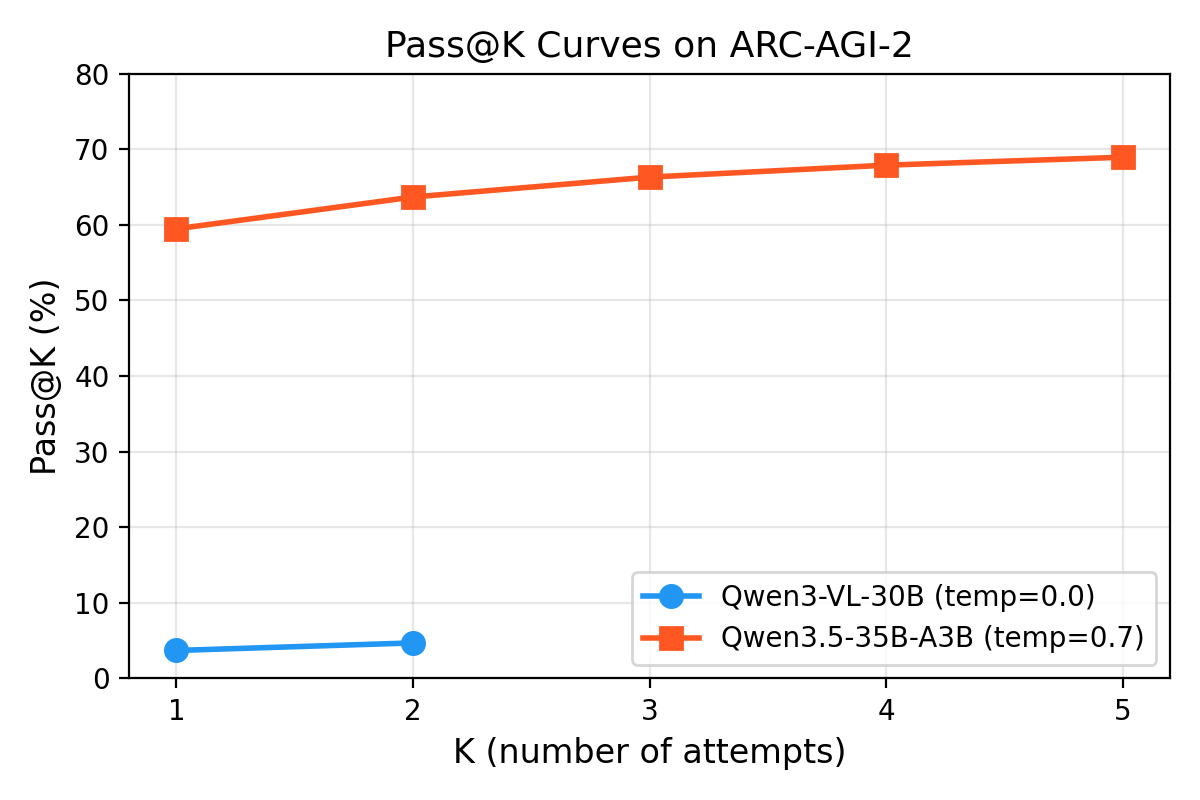
\includegraphics[width=0.75\textwidth]{passk_curve.png}
\caption{Pass@K curves on ARC-AGI-2. Qwen3-VL results (on ARC-AGI-1) are shown for reference only and are not directly comparable due to different benchmarks and settings.}
\label{fig:passk}
\end{figure}

\subsubsection{Prompt Token Analysis}
The relationship between prompt length and task success is further analyzed. Tasks with shorter prompts exhibit higher success rates than tasks with longer prompts (Figure~\ref{fig:prompt_tokens}). However, this correlation should be interpreted with caution: longer prompts correspond to tasks with larger grids, which are inherently more difficult. The observed relationship is therefore likely a confounding effect of task complexity rather than a direct causal relationship between prompt length and model performance.

\begin{figure}[H]
\centering
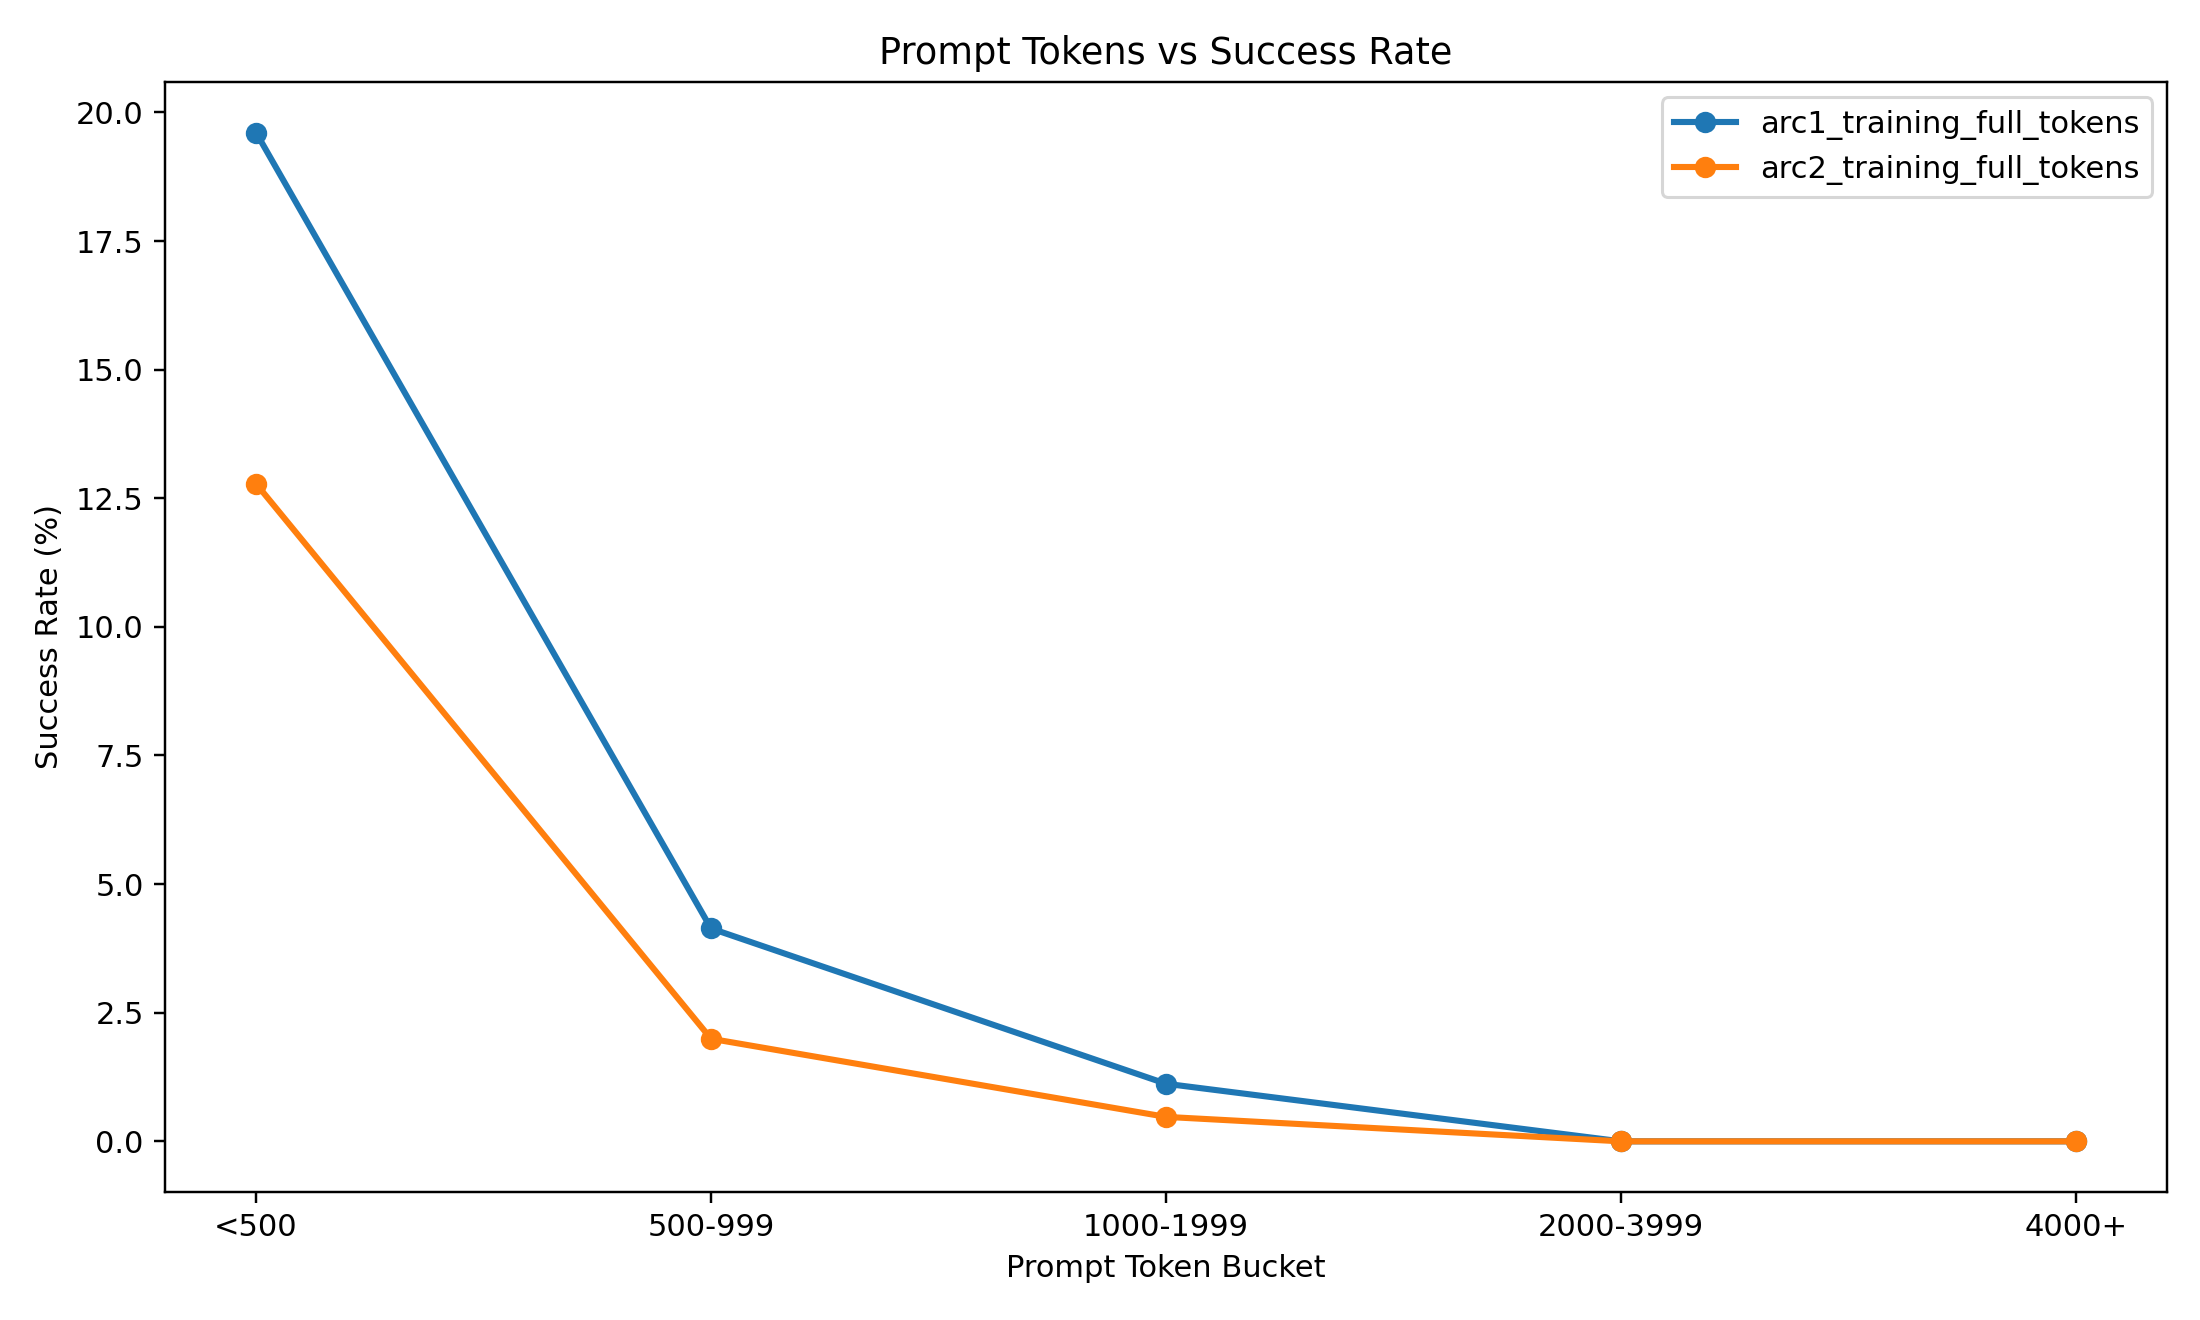
\includegraphics[width=0.8\textwidth]{03_prompt_tokens_vs_success.png}
\caption{Distribution of prompt token counts across ARC tasks for ARC-AGI-1 and ARC-AGI-2. 
ARC-AGI-2 tasks generally require longer prompts due to increased task complexity.}
\label{fig:prompt_tokens}
\end{figure}

\subsubsection{Failure Mode Analysis}
Failure cases are categorized according to per-task final outcome. For Qwen3.5, out of 190 tasks, 49 (25.8\%) result in training failure (the program does not reproduce the training examples), 10 (5.3\%) produce wrong output on test inputs despite passing training, and 131 (68.9\%) are solved correctly (Figure~\ref{fig:failure_modes}).

\begin{figure}[H]
\centering
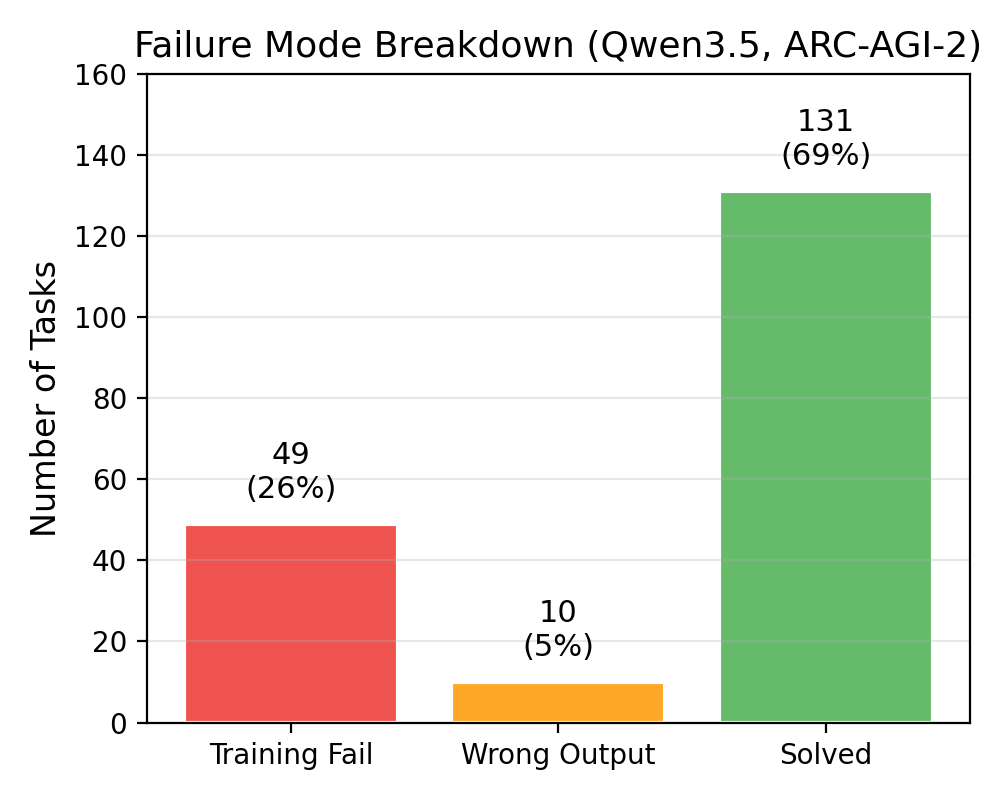
\includegraphics[width=0.65\textwidth]{failure_modes.png}
\caption{Failure mode breakdown for Qwen3.5 on ARC-AGI-2 (190 tasks). Training failure dominates, indicating that inferring the correct rule remains the primary challenge.}
\label{fig:failure_modes}
\end{figure}

Training failure remains the dominant failure mode, suggesting that the model frequently fails to infer the correct transformation rule from the few-shot examples. Notably, in the wrong-output cases, cell-level accuracy is high (mean 89.8\%, median 97.8\%), indicating that the model often captures most of the transformation rule but makes errors on edge cases or specific grid cells. This near-miss behavior suggests that partial credit reward shaping could provide useful learning signal for RL training.

\subsubsection{How These Results Support Our Claim}
The experimental results yield several key observations that support the feasibility of our proposed RL approach.

Most importantly, the 59.5\% pass@1 rate of Qwen3.5-35B-A3B on ARC-AGI-2 demonstrates that the reward signal is not too sparse for RL training---a majority of sampled programs receive positive reward on the first attempt, which is essential for GRPO to produce meaningful policy gradients. This is a critical prerequisite: if the base model rarely produced correct solutions, the RL reward signal would be too sparse to learn from.

Retry analysis shows diminishing but meaningful returns from additional attempts, indicating that the model can benefit from execution feedback but does not yet have an effective mechanism to systematically leverage it. Failure mode analysis reveals that training failure (failing to reproduce training examples) remains the dominant failure mode at 25.8\% of tasks, confirming that inferring the correct transformation rule is the primary challenge. The high cell accuracy in wrong-output cases (median 97.8\%) further suggests that partial credit reward shaping could provide additional gradient signal beyond binary correctness.

These findings motivate the proposed reinforcement learning framework, which utilizes execution outcomes as reward signals to improve the model's capacity for rule inference and iterative solution refinement.



\section{Future milestones}
{\color{red}
\begin{enumerate}
    \item Dates and sub-goals (please set sub-goals on a weekly basis so that they can be done in a week).
\end{enumerate}
}
March 16 - March 29:\\
Build the GRPO training pipeline for ARC, including code generation, code execution, reward calculation, and feedback collection. Run small-scale experiments to check whether training is stable.
\\\\
March 30 - April 12:\\
Tune the reward function and training settings, and run training on a larger set of ARC tasks to improve model performance.
\\\\
April 13 - April 30:\\
Evaluate the trained model on ARC-AGI-1 and ARC-AGI-2, analyze the final results, and prepare the final report and presentation.
\section{Conclusion}
{\color{red}
\begin{enumerate}
    \item Summary of your progress and your final expected goal (what do you expect to achieve or demonstrate for the final project?).
\end{enumerate}
}
In this project, we explore how to improve LLM-based code generation for ARC using reinforcement learning with execution feedback. ARC is difficult because it requires the model to infer abstract rules from only a few examples, which is still challenging for current LLMs. Our method uses GRPO to train the model based on whether the generated code is correct, executable, and able to improve through feedback.
\\ \\
So far, we have finished the baseline experiments and identified the main problem: prompting alone is not enough for strong reasoning and self-correction on ARC. Our early experiments with Qwen3.5-35B-A3B show that the reward is not too sparse---the model achieves 59.5\% pass@1 on ARC-AGI-2 tasks, providing a substantial fraction of positive reward signals for GRPO training. Furthermore, the high cell accuracy in near-miss cases (median 97.8\%) suggests that partial credit reward shaping could provide additional gradient signal. For the final project, we hope to show that this training method can improve the model’s pass@1 accuracy and help it generate more correct programs for ARC tasks.

\section{Author Contributions}
{\color{red}
\begin{enumerate}
    \item Please see the guideline "Contribution of each team member" below.
\end{enumerate}
}

\newpage
% Refernces
\bibliographystyle{unsrtnat}
\bibliography{ref}

\end{document}